\documentclass[11pt]{article}

    \usepackage[breakable]{tcolorbox}
    \usepackage{parskip} % Stop auto-indenting (to mimic markdown behaviour)
    

    % Basic figure setup, for now with no caption control since it's done
    % automatically by Pandoc (which extracts ![](path) syntax from Markdown).
    \usepackage{graphicx}
    % Maintain compatibility with old templates. Remove in nbconvert 6.0
    \let\Oldincludegraphics\includegraphics
    % Ensure that by default, figures have no caption (until we provide a
    % proper Figure object with a Caption API and a way to capture that
    % in the conversion process - todo).
    \usepackage{caption}
    \DeclareCaptionFormat{nocaption}{}
    \captionsetup{format=nocaption,aboveskip=0pt,belowskip=0pt}

    \usepackage{float}
    \floatplacement{figure}{H} % forces figures to be placed at the correct location
    \usepackage{xcolor} % Allow colors to be defined
    \usepackage{enumerate} % Needed for markdown enumerations to work
    \usepackage{geometry} % Used to adjust the document margins
    \usepackage{amsmath} % Equations
    \usepackage{amssymb} % Equations
    \usepackage{textcomp} % defines textquotesingle
    % Hack from http://tex.stackexchange.com/a/47451/13684:
    \AtBeginDocument{%
        \def\PYZsq{\textquotesingle}% Upright quotes in Pygmentized code
    }
    \usepackage{upquote} % Upright quotes for verbatim code
    \usepackage{eurosym} % defines \euro

    \usepackage{iftex}
    \ifPDFTeX
        \usepackage[T1]{fontenc}
        \IfFileExists{alphabeta.sty}{
              \usepackage{alphabeta}
          }{
              \usepackage[mathletters]{ucs}
              \usepackage[utf8x]{inputenc}
          }
    \else
        \usepackage{fontspec}
        \usepackage{unicode-math}
    \fi

    \usepackage{fancyvrb} % verbatim replacement that allows latex
    \usepackage{grffile} % extends the file name processing of package graphics
                         % to support a larger range
    \makeatletter % fix for old versions of grffile with XeLaTeX
    \@ifpackagelater{grffile}{2019/11/01}
    {
      % Do nothing on new versions
    }
    {
      \def\Gread@@xetex#1{%
        \IfFileExists{"\Gin@base".bb}%
        {\Gread@eps{\Gin@base.bb}}%
        {\Gread@@xetex@aux#1}%
      }
    }
    \makeatother
    \usepackage[Export]{adjustbox} % Used to constrain images to a maximum size
    \adjustboxset{max size={0.9\linewidth}{0.9\paperheight}}

    % The hyperref package gives us a pdf with properly built
    % internal navigation ('pdf bookmarks' for the table of contents,
    % internal cross-reference links, web links for URLs, etc.)
    \usepackage{hyperref}
    % The default LaTeX title has an obnoxious amount of whitespace. By default,
    % titling removes some of it. It also provides customization options.
    \usepackage{titling}
    \usepackage{longtable} % longtable support required by pandoc >1.10
    \usepackage{booktabs}  % table support for pandoc > 1.12.2
    \usepackage{array}     % table support for pandoc >= 2.11.3
    \usepackage{calc}      % table minipage width calculation for pandoc >= 2.11.1
    \usepackage[inline]{enumitem} % IRkernel/repr support (it uses the enumerate* environment)
    \usepackage[normalem]{ulem} % ulem is needed to support strikethroughs (\sout)
                                % normalem makes italics be italics, not underlines
    \usepackage{mathrsfs}
    

    
    % Colors for the hyperref package
    \definecolor{urlcolor}{rgb}{0,.145,.698}
    \definecolor{linkcolor}{rgb}{.71,0.21,0.01}
    \definecolor{citecolor}{rgb}{.12,.54,.11}

    % ANSI colors
    \definecolor{ansi-black}{HTML}{3E424D}
    \definecolor{ansi-black-intense}{HTML}{282C36}
    \definecolor{ansi-red}{HTML}{E75C58}
    \definecolor{ansi-red-intense}{HTML}{B22B31}
    \definecolor{ansi-green}{HTML}{00A250}
    \definecolor{ansi-green-intense}{HTML}{007427}
    \definecolor{ansi-yellow}{HTML}{DDB62B}
    \definecolor{ansi-yellow-intense}{HTML}{B27D12}
    \definecolor{ansi-blue}{HTML}{208FFB}
    \definecolor{ansi-blue-intense}{HTML}{0065CA}
    \definecolor{ansi-magenta}{HTML}{D160C4}
    \definecolor{ansi-magenta-intense}{HTML}{A03196}
    \definecolor{ansi-cyan}{HTML}{60C6C8}
    \definecolor{ansi-cyan-intense}{HTML}{258F8F}
    \definecolor{ansi-white}{HTML}{C5C1B4}
    \definecolor{ansi-white-intense}{HTML}{A1A6B2}
    \definecolor{ansi-default-inverse-fg}{HTML}{FFFFFF}
    \definecolor{ansi-default-inverse-bg}{HTML}{000000}

    % common color for the border for error outputs.
    \definecolor{outerrorbackground}{HTML}{FFDFDF}

    % commands and environments needed by pandoc snippets
    % extracted from the output of `pandoc -s`
    \providecommand{\tightlist}{%
      \setlength{\itemsep}{0pt}\setlength{\parskip}{0pt}}
    \DefineVerbatimEnvironment{Highlighting}{Verbatim}{commandchars=\\\{\}}
    % Add ',fontsize=\small' for more characters per line
    \newenvironment{Shaded}{}{}
    \newcommand{\KeywordTok}[1]{\textcolor[rgb]{0.00,0.44,0.13}{\textbf{{#1}}}}
    \newcommand{\DataTypeTok}[1]{\textcolor[rgb]{0.56,0.13,0.00}{{#1}}}
    \newcommand{\DecValTok}[1]{\textcolor[rgb]{0.25,0.63,0.44}{{#1}}}
    \newcommand{\BaseNTok}[1]{\textcolor[rgb]{0.25,0.63,0.44}{{#1}}}
    \newcommand{\FloatTok}[1]{\textcolor[rgb]{0.25,0.63,0.44}{{#1}}}
    \newcommand{\CharTok}[1]{\textcolor[rgb]{0.25,0.44,0.63}{{#1}}}
    \newcommand{\StringTok}[1]{\textcolor[rgb]{0.25,0.44,0.63}{{#1}}}
    \newcommand{\CommentTok}[1]{\textcolor[rgb]{0.38,0.63,0.69}{\textit{{#1}}}}
    \newcommand{\OtherTok}[1]{\textcolor[rgb]{0.00,0.44,0.13}{{#1}}}
    \newcommand{\AlertTok}[1]{\textcolor[rgb]{1.00,0.00,0.00}{\textbf{{#1}}}}
    \newcommand{\FunctionTok}[1]{\textcolor[rgb]{0.02,0.16,0.49}{{#1}}}
    \newcommand{\RegionMarkerTok}[1]{{#1}}
    \newcommand{\ErrorTok}[1]{\textcolor[rgb]{1.00,0.00,0.00}{\textbf{{#1}}}}
    \newcommand{\NormalTok}[1]{{#1}}

    % Additional commands for more recent versions of Pandoc
    \newcommand{\ConstantTok}[1]{\textcolor[rgb]{0.53,0.00,0.00}{{#1}}}
    \newcommand{\SpecialCharTok}[1]{\textcolor[rgb]{0.25,0.44,0.63}{{#1}}}
    \newcommand{\VerbatimStringTok}[1]{\textcolor[rgb]{0.25,0.44,0.63}{{#1}}}
    \newcommand{\SpecialStringTok}[1]{\textcolor[rgb]{0.73,0.40,0.53}{{#1}}}
    \newcommand{\ImportTok}[1]{{#1}}
    \newcommand{\DocumentationTok}[1]{\textcolor[rgb]{0.73,0.13,0.13}{\textit{{#1}}}}
    \newcommand{\AnnotationTok}[1]{\textcolor[rgb]{0.38,0.63,0.69}{\textbf{\textit{{#1}}}}}
    \newcommand{\CommentVarTok}[1]{\textcolor[rgb]{0.38,0.63,0.69}{\textbf{\textit{{#1}}}}}
    \newcommand{\VariableTok}[1]{\textcolor[rgb]{0.10,0.09,0.49}{{#1}}}
    \newcommand{\ControlFlowTok}[1]{\textcolor[rgb]{0.00,0.44,0.13}{\textbf{{#1}}}}
    \newcommand{\OperatorTok}[1]{\textcolor[rgb]{0.40,0.40,0.40}{{#1}}}
    \newcommand{\BuiltInTok}[1]{{#1}}
    \newcommand{\ExtensionTok}[1]{{#1}}
    \newcommand{\PreprocessorTok}[1]{\textcolor[rgb]{0.74,0.48,0.00}{{#1}}}
    \newcommand{\AttributeTok}[1]{\textcolor[rgb]{0.49,0.56,0.16}{{#1}}}
    \newcommand{\InformationTok}[1]{\textcolor[rgb]{0.38,0.63,0.69}{\textbf{\textit{{#1}}}}}
    \newcommand{\WarningTok}[1]{\textcolor[rgb]{0.38,0.63,0.69}{\textbf{\textit{{#1}}}}}


    % Define a nice break command that doesn't care if a line doesn't already
    % exist.
    \def\br{\hspace*{\fill} \\* }
    % Math Jax compatibility definitions
    \def\gt{>}
    \def\lt{<}
    \let\Oldtex\TeX
    \let\Oldlatex\LaTeX
    \renewcommand{\TeX}{\textrm{\Oldtex}}
    \renewcommand{\LaTeX}{\textrm{\Oldlatex}}
    % Document parameters
    % Document title
    \title{Untitled}
    
    
    
    
    
% Pygments definitions
\makeatletter
\def\PY@reset{\let\PY@it=\relax \let\PY@bf=\relax%
    \let\PY@ul=\relax \let\PY@tc=\relax%
    \let\PY@bc=\relax \let\PY@ff=\relax}
\def\PY@tok#1{\csname PY@tok@#1\endcsname}
\def\PY@toks#1+{\ifx\relax#1\empty\else%
    \PY@tok{#1}\expandafter\PY@toks\fi}
\def\PY@do#1{\PY@bc{\PY@tc{\PY@ul{%
    \PY@it{\PY@bf{\PY@ff{#1}}}}}}}
\def\PY#1#2{\PY@reset\PY@toks#1+\relax+\PY@do{#2}}

\@namedef{PY@tok@w}{\def\PY@tc##1{\textcolor[rgb]{0.73,0.73,0.73}{##1}}}
\@namedef{PY@tok@c}{\let\PY@it=\textit\def\PY@tc##1{\textcolor[rgb]{0.24,0.48,0.48}{##1}}}
\@namedef{PY@tok@cp}{\def\PY@tc##1{\textcolor[rgb]{0.61,0.40,0.00}{##1}}}
\@namedef{PY@tok@k}{\let\PY@bf=\textbf\def\PY@tc##1{\textcolor[rgb]{0.00,0.50,0.00}{##1}}}
\@namedef{PY@tok@kp}{\def\PY@tc##1{\textcolor[rgb]{0.00,0.50,0.00}{##1}}}
\@namedef{PY@tok@kt}{\def\PY@tc##1{\textcolor[rgb]{0.69,0.00,0.25}{##1}}}
\@namedef{PY@tok@o}{\def\PY@tc##1{\textcolor[rgb]{0.40,0.40,0.40}{##1}}}
\@namedef{PY@tok@ow}{\let\PY@bf=\textbf\def\PY@tc##1{\textcolor[rgb]{0.67,0.13,1.00}{##1}}}
\@namedef{PY@tok@nb}{\def\PY@tc##1{\textcolor[rgb]{0.00,0.50,0.00}{##1}}}
\@namedef{PY@tok@nf}{\def\PY@tc##1{\textcolor[rgb]{0.00,0.00,1.00}{##1}}}
\@namedef{PY@tok@nc}{\let\PY@bf=\textbf\def\PY@tc##1{\textcolor[rgb]{0.00,0.00,1.00}{##1}}}
\@namedef{PY@tok@nn}{\let\PY@bf=\textbf\def\PY@tc##1{\textcolor[rgb]{0.00,0.00,1.00}{##1}}}
\@namedef{PY@tok@ne}{\let\PY@bf=\textbf\def\PY@tc##1{\textcolor[rgb]{0.80,0.25,0.22}{##1}}}
\@namedef{PY@tok@nv}{\def\PY@tc##1{\textcolor[rgb]{0.10,0.09,0.49}{##1}}}
\@namedef{PY@tok@no}{\def\PY@tc##1{\textcolor[rgb]{0.53,0.00,0.00}{##1}}}
\@namedef{PY@tok@nl}{\def\PY@tc##1{\textcolor[rgb]{0.46,0.46,0.00}{##1}}}
\@namedef{PY@tok@ni}{\let\PY@bf=\textbf\def\PY@tc##1{\textcolor[rgb]{0.44,0.44,0.44}{##1}}}
\@namedef{PY@tok@na}{\def\PY@tc##1{\textcolor[rgb]{0.41,0.47,0.13}{##1}}}
\@namedef{PY@tok@nt}{\let\PY@bf=\textbf\def\PY@tc##1{\textcolor[rgb]{0.00,0.50,0.00}{##1}}}
\@namedef{PY@tok@nd}{\def\PY@tc##1{\textcolor[rgb]{0.67,0.13,1.00}{##1}}}
\@namedef{PY@tok@s}{\def\PY@tc##1{\textcolor[rgb]{0.73,0.13,0.13}{##1}}}
\@namedef{PY@tok@sd}{\let\PY@it=\textit\def\PY@tc##1{\textcolor[rgb]{0.73,0.13,0.13}{##1}}}
\@namedef{PY@tok@si}{\let\PY@bf=\textbf\def\PY@tc##1{\textcolor[rgb]{0.64,0.35,0.47}{##1}}}
\@namedef{PY@tok@se}{\let\PY@bf=\textbf\def\PY@tc##1{\textcolor[rgb]{0.67,0.36,0.12}{##1}}}
\@namedef{PY@tok@sr}{\def\PY@tc##1{\textcolor[rgb]{0.64,0.35,0.47}{##1}}}
\@namedef{PY@tok@ss}{\def\PY@tc##1{\textcolor[rgb]{0.10,0.09,0.49}{##1}}}
\@namedef{PY@tok@sx}{\def\PY@tc##1{\textcolor[rgb]{0.00,0.50,0.00}{##1}}}
\@namedef{PY@tok@m}{\def\PY@tc##1{\textcolor[rgb]{0.40,0.40,0.40}{##1}}}
\@namedef{PY@tok@gh}{\let\PY@bf=\textbf\def\PY@tc##1{\textcolor[rgb]{0.00,0.00,0.50}{##1}}}
\@namedef{PY@tok@gu}{\let\PY@bf=\textbf\def\PY@tc##1{\textcolor[rgb]{0.50,0.00,0.50}{##1}}}
\@namedef{PY@tok@gd}{\def\PY@tc##1{\textcolor[rgb]{0.63,0.00,0.00}{##1}}}
\@namedef{PY@tok@gi}{\def\PY@tc##1{\textcolor[rgb]{0.00,0.52,0.00}{##1}}}
\@namedef{PY@tok@gr}{\def\PY@tc##1{\textcolor[rgb]{0.89,0.00,0.00}{##1}}}
\@namedef{PY@tok@ge}{\let\PY@it=\textit}
\@namedef{PY@tok@gs}{\let\PY@bf=\textbf}
\@namedef{PY@tok@gp}{\let\PY@bf=\textbf\def\PY@tc##1{\textcolor[rgb]{0.00,0.00,0.50}{##1}}}
\@namedef{PY@tok@go}{\def\PY@tc##1{\textcolor[rgb]{0.44,0.44,0.44}{##1}}}
\@namedef{PY@tok@gt}{\def\PY@tc##1{\textcolor[rgb]{0.00,0.27,0.87}{##1}}}
\@namedef{PY@tok@err}{\def\PY@bc##1{{\setlength{\fboxsep}{\string -\fboxrule}\fcolorbox[rgb]{1.00,0.00,0.00}{1,1,1}{\strut ##1}}}}
\@namedef{PY@tok@kc}{\let\PY@bf=\textbf\def\PY@tc##1{\textcolor[rgb]{0.00,0.50,0.00}{##1}}}
\@namedef{PY@tok@kd}{\let\PY@bf=\textbf\def\PY@tc##1{\textcolor[rgb]{0.00,0.50,0.00}{##1}}}
\@namedef{PY@tok@kn}{\let\PY@bf=\textbf\def\PY@tc##1{\textcolor[rgb]{0.00,0.50,0.00}{##1}}}
\@namedef{PY@tok@kr}{\let\PY@bf=\textbf\def\PY@tc##1{\textcolor[rgb]{0.00,0.50,0.00}{##1}}}
\@namedef{PY@tok@bp}{\def\PY@tc##1{\textcolor[rgb]{0.00,0.50,0.00}{##1}}}
\@namedef{PY@tok@fm}{\def\PY@tc##1{\textcolor[rgb]{0.00,0.00,1.00}{##1}}}
\@namedef{PY@tok@vc}{\def\PY@tc##1{\textcolor[rgb]{0.10,0.09,0.49}{##1}}}
\@namedef{PY@tok@vg}{\def\PY@tc##1{\textcolor[rgb]{0.10,0.09,0.49}{##1}}}
\@namedef{PY@tok@vi}{\def\PY@tc##1{\textcolor[rgb]{0.10,0.09,0.49}{##1}}}
\@namedef{PY@tok@vm}{\def\PY@tc##1{\textcolor[rgb]{0.10,0.09,0.49}{##1}}}
\@namedef{PY@tok@sa}{\def\PY@tc##1{\textcolor[rgb]{0.73,0.13,0.13}{##1}}}
\@namedef{PY@tok@sb}{\def\PY@tc##1{\textcolor[rgb]{0.73,0.13,0.13}{##1}}}
\@namedef{PY@tok@sc}{\def\PY@tc##1{\textcolor[rgb]{0.73,0.13,0.13}{##1}}}
\@namedef{PY@tok@dl}{\def\PY@tc##1{\textcolor[rgb]{0.73,0.13,0.13}{##1}}}
\@namedef{PY@tok@s2}{\def\PY@tc##1{\textcolor[rgb]{0.73,0.13,0.13}{##1}}}
\@namedef{PY@tok@sh}{\def\PY@tc##1{\textcolor[rgb]{0.73,0.13,0.13}{##1}}}
\@namedef{PY@tok@s1}{\def\PY@tc##1{\textcolor[rgb]{0.73,0.13,0.13}{##1}}}
\@namedef{PY@tok@mb}{\def\PY@tc##1{\textcolor[rgb]{0.40,0.40,0.40}{##1}}}
\@namedef{PY@tok@mf}{\def\PY@tc##1{\textcolor[rgb]{0.40,0.40,0.40}{##1}}}
\@namedef{PY@tok@mh}{\def\PY@tc##1{\textcolor[rgb]{0.40,0.40,0.40}{##1}}}
\@namedef{PY@tok@mi}{\def\PY@tc##1{\textcolor[rgb]{0.40,0.40,0.40}{##1}}}
\@namedef{PY@tok@il}{\def\PY@tc##1{\textcolor[rgb]{0.40,0.40,0.40}{##1}}}
\@namedef{PY@tok@mo}{\def\PY@tc##1{\textcolor[rgb]{0.40,0.40,0.40}{##1}}}
\@namedef{PY@tok@ch}{\let\PY@it=\textit\def\PY@tc##1{\textcolor[rgb]{0.24,0.48,0.48}{##1}}}
\@namedef{PY@tok@cm}{\let\PY@it=\textit\def\PY@tc##1{\textcolor[rgb]{0.24,0.48,0.48}{##1}}}
\@namedef{PY@tok@cpf}{\let\PY@it=\textit\def\PY@tc##1{\textcolor[rgb]{0.24,0.48,0.48}{##1}}}
\@namedef{PY@tok@c1}{\let\PY@it=\textit\def\PY@tc##1{\textcolor[rgb]{0.24,0.48,0.48}{##1}}}
\@namedef{PY@tok@cs}{\let\PY@it=\textit\def\PY@tc##1{\textcolor[rgb]{0.24,0.48,0.48}{##1}}}

\def\PYZbs{\char`\\}
\def\PYZus{\char`\_}
\def\PYZob{\char`\{}
\def\PYZcb{\char`\}}
\def\PYZca{\char`\^}
\def\PYZam{\char`\&}
\def\PYZlt{\char`\<}
\def\PYZgt{\char`\>}
\def\PYZsh{\char`\#}
\def\PYZpc{\char`\%}
\def\PYZdl{\char`\$}
\def\PYZhy{\char`\-}
\def\PYZsq{\char`\'}
\def\PYZdq{\char`\"}
\def\PYZti{\char`\~}
% for compatibility with earlier versions
\def\PYZat{@}
\def\PYZlb{[}
\def\PYZrb{]}
\makeatother


    % For linebreaks inside Verbatim environment from package fancyvrb.
    \makeatletter
        \newbox\Wrappedcontinuationbox
        \newbox\Wrappedvisiblespacebox
        \newcommand*\Wrappedvisiblespace {\textcolor{red}{\textvisiblespace}}
        \newcommand*\Wrappedcontinuationsymbol {\textcolor{red}{\llap{\tiny$\m@th\hookrightarrow$}}}
        \newcommand*\Wrappedcontinuationindent {3ex }
        \newcommand*\Wrappedafterbreak {\kern\Wrappedcontinuationindent\copy\Wrappedcontinuationbox}
        % Take advantage of the already applied Pygments mark-up to insert
        % potential linebreaks for TeX processing.
        %        {, <, #, %, $, ' and ": go to next line.
        %        _, }, ^, &, >, - and ~: stay at end of broken line.
        % Use of \textquotesingle for straight quote.
        \newcommand*\Wrappedbreaksatspecials {%
            \def\PYGZus{\discretionary{\char`\_}{\Wrappedafterbreak}{\char`\_}}%
            \def\PYGZob{\discretionary{}{\Wrappedafterbreak\char`\{}{\char`\{}}%
            \def\PYGZcb{\discretionary{\char`\}}{\Wrappedafterbreak}{\char`\}}}%
            \def\PYGZca{\discretionary{\char`\^}{\Wrappedafterbreak}{\char`\^}}%
            \def\PYGZam{\discretionary{\char`\&}{\Wrappedafterbreak}{\char`\&}}%
            \def\PYGZlt{\discretionary{}{\Wrappedafterbreak\char`\<}{\char`\<}}%
            \def\PYGZgt{\discretionary{\char`\>}{\Wrappedafterbreak}{\char`\>}}%
            \def\PYGZsh{\discretionary{}{\Wrappedafterbreak\char`\#}{\char`\#}}%
            \def\PYGZpc{\discretionary{}{\Wrappedafterbreak\char`\%}{\char`\%}}%
            \def\PYGZdl{\discretionary{}{\Wrappedafterbreak\char`\$}{\char`\$}}%
            \def\PYGZhy{\discretionary{\char`\-}{\Wrappedafterbreak}{\char`\-}}%
            \def\PYGZsq{\discretionary{}{\Wrappedafterbreak\textquotesingle}{\textquotesingle}}%
            \def\PYGZdq{\discretionary{}{\Wrappedafterbreak\char`\"}{\char`\"}}%
            \def\PYGZti{\discretionary{\char`\~}{\Wrappedafterbreak}{\char`\~}}%
        }
        % Some characters . , ; ? ! / are not pygmentized.
        % This macro makes them "active" and they will insert potential linebreaks
        \newcommand*\Wrappedbreaksatpunct {%
            \lccode`\~`\.\lowercase{\def~}{\discretionary{\hbox{\char`\.}}{\Wrappedafterbreak}{\hbox{\char`\.}}}%
            \lccode`\~`\,\lowercase{\def~}{\discretionary{\hbox{\char`\,}}{\Wrappedafterbreak}{\hbox{\char`\,}}}%
            \lccode`\~`\;\lowercase{\def~}{\discretionary{\hbox{\char`\;}}{\Wrappedafterbreak}{\hbox{\char`\;}}}%
            \lccode`\~`\:\lowercase{\def~}{\discretionary{\hbox{\char`\:}}{\Wrappedafterbreak}{\hbox{\char`\:}}}%
            \lccode`\~`\?\lowercase{\def~}{\discretionary{\hbox{\char`\?}}{\Wrappedafterbreak}{\hbox{\char`\?}}}%
            \lccode`\~`\!\lowercase{\def~}{\discretionary{\hbox{\char`\!}}{\Wrappedafterbreak}{\hbox{\char`\!}}}%
            \lccode`\~`\/\lowercase{\def~}{\discretionary{\hbox{\char`\/}}{\Wrappedafterbreak}{\hbox{\char`\/}}}%
            \catcode`\.\active
            \catcode`\,\active
            \catcode`\;\active
            \catcode`\:\active
            \catcode`\?\active
            \catcode`\!\active
            \catcode`\/\active
            \lccode`\~`\~
        }
    \makeatother

    \let\OriginalVerbatim=\Verbatim
    \makeatletter
    \renewcommand{\Verbatim}[1][1]{%
        %\parskip\z@skip
        \sbox\Wrappedcontinuationbox {\Wrappedcontinuationsymbol}%
        \sbox\Wrappedvisiblespacebox {\FV@SetupFont\Wrappedvisiblespace}%
        \def\FancyVerbFormatLine ##1{\hsize\linewidth
            \vtop{\raggedright\hyphenpenalty\z@\exhyphenpenalty\z@
                \doublehyphendemerits\z@\finalhyphendemerits\z@
                \strut ##1\strut}%
        }%
        % If the linebreak is at a space, the latter will be displayed as visible
        % space at end of first line, and a continuation symbol starts next line.
        % Stretch/shrink are however usually zero for typewriter font.
        \def\FV@Space {%
            \nobreak\hskip\z@ plus\fontdimen3\font minus\fontdimen4\font
            \discretionary{\copy\Wrappedvisiblespacebox}{\Wrappedafterbreak}
            {\kern\fontdimen2\font}%
        }%

        % Allow breaks at special characters using \PYG... macros.
        \Wrappedbreaksatspecials
        % Breaks at punctuation characters . , ; ? ! and / need catcode=\active
        \OriginalVerbatim[#1,codes*=\Wrappedbreaksatpunct]%
    }
    \makeatother

    % Exact colors from NB
    \definecolor{incolor}{HTML}{303F9F}
    \definecolor{outcolor}{HTML}{D84315}
    \definecolor{cellborder}{HTML}{CFCFCF}
    \definecolor{cellbackground}{HTML}{F7F7F7}

    % prompt
    \makeatletter
    \newcommand{\boxspacing}{\kern\kvtcb@left@rule\kern\kvtcb@boxsep}
    \makeatother
    \newcommand{\prompt}[4]{
        {\ttfamily\llap{{\color{#2}[#3]:\hspace{3pt}#4}}\vspace{-\baselineskip}}
    }
    

    
    % Prevent overflowing lines due to hard-to-break entities
    \sloppy
    % Setup hyperref package
    \hypersetup{
      breaklinks=true,  % so long urls are correctly broken across lines
      colorlinks=true,
      urlcolor=urlcolor,
      linkcolor=linkcolor,
      citecolor=citecolor,
      }
    % Slightly bigger margins than the latex defaults
    
    \geometry{verbose,tmargin=1in,bmargin=1in,lmargin=1in,rmargin=1in}
    
    

\begin{document}
    
    \maketitle
    
    

    
    \hypertarget{covid-19-muxe9xico-en-datos}{%
\section{COVID-19: México en Datos}\label{covid-19-muxe9xico-en-datos}}

\hypertarget{introducciuxf3n}{%
\section{Introducción}\label{introducciuxf3n}}

En el presente trabajo se analizará el repositorio de datos abiertos de
la Secretaría de Salud Federal referentes a la pandemia de COVID-19
durante el año 2021 en nuestro país.

La fuente de los datos es la misma Secretaría de Salud, en su apartado
de
\href{https://www.gob.mx/salud/documentos/datos-abiertos-152127}{datos
abiertos}. Para este análisis, tomamos los datos históricos del 2021,
los cuales se encuentran almacenados en un archivo .csv (valores
separados por comas) con un peso aproximado de 1.5 Gb. Este archivo
contiene todos los datos sospechosos de covid registrados en
instituciones médicas del país entre el 1 de enero de 2021 y el 29 de
julio de 2022.

Cada fila en esta base representa un paciente admitido en un Centro
Médico del país por posible contagio de COVID-19. Las diferentes
columnas representan diversas características o padecimientos del
paciente, tales como su lugar de residencia, de nacimiento, la ubicación
de la unidad médica donde se atendió y si era una institución pública o
privada, si sufría de diabetes, hipertensión, EPOC, u otras condiciones,
si pertenecía a una comunidad indígena, entre otros.

\hypertarget{explorando-los-datos}{%
\section{Explorando los datos}\label{explorando-los-datos}}

\hypertarget{estructura-de-la-base-de-datos}{%
\subsection{Estructura de la Base de
Datos}\label{estructura-de-la-base-de-datos}}

Para generar nuestra base de datos MySQL, utilizaremos un único archivo
csv proporcionado por la Secretaría de Salud. Sin embargo, utilizando el
diccionario de datos proporcionado por la misma Secretaría, podemos
generar tablas adicionales para complementar nuestra tabla principal.
Una vez realizado este proceso, nuestra base de datos contaría con la
siguiente estructura.

\begin{figure}
\centering
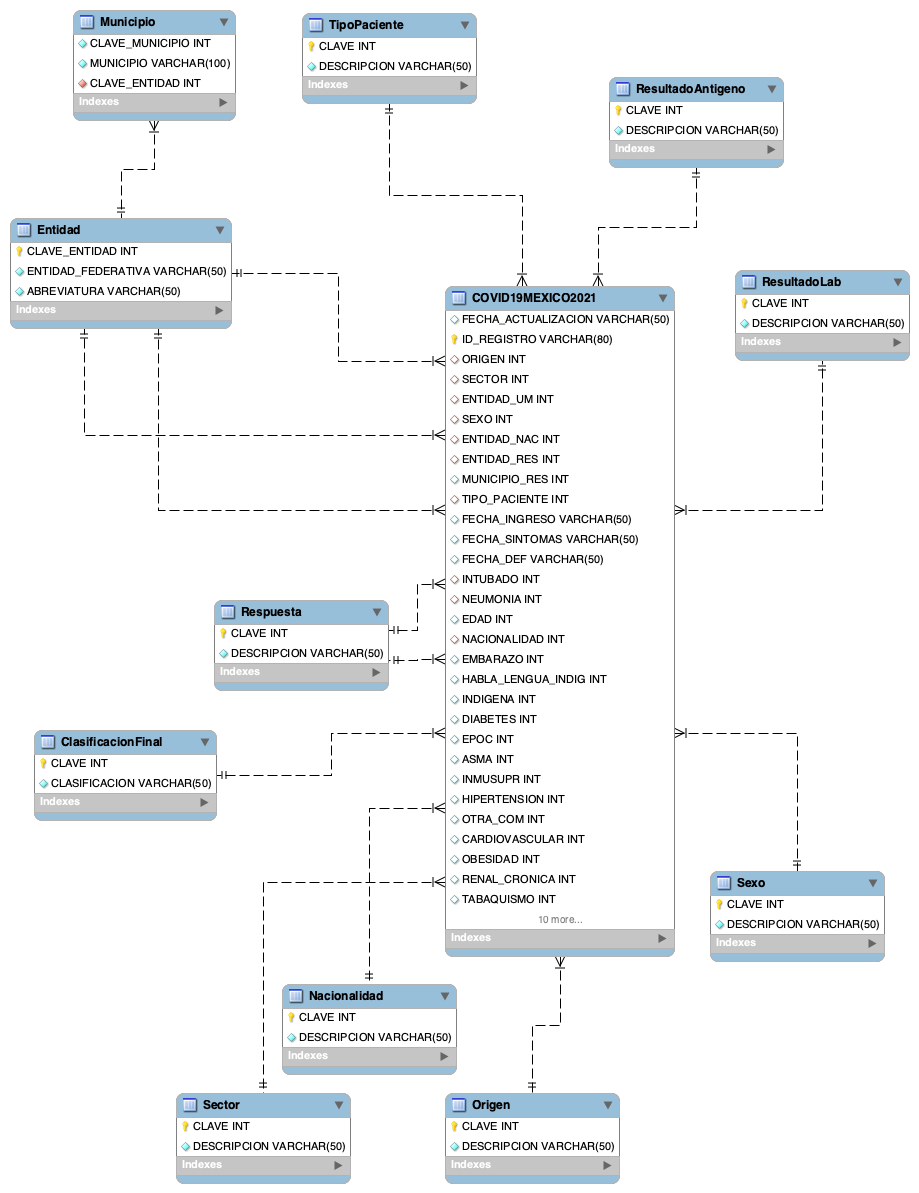
\includegraphics{./img/diagrama.png}
\caption{Diagram ER de la base de datos}
\end{figure}

Estas relaciones nos permitirán, como veremos más adelante, analizar e
interpretar más facilmente los datos que recabaremos con nuestras
queries. Las queries utilizadas estarán disponibles en el repositorio
del proyecto.

\hypertarget{analizando-los-datos-de-nuestra-base}{%
\subsection{Analizando los datos de nuestra
base}\label{analizando-los-datos-de-nuestra-base}}

\hypertarget{cuuxe1ntos-casos-registruxf3-la-secretaruxeda}{%
\subsubsection{¿Cuántos casos registró la
Secretaría?}\label{cuuxe1ntos-casos-registruxf3-la-secretaruxeda}}

Comenzamos analizando la cantidad total de registros en nuestra tabla
principal, para eso podemos utilizar una query simple utilizando la
función COUNT.

\begin{Shaded}
\begin{Highlighting}[]
\KeywordTok{SELECT} 
    \FunctionTok{COUNT}\NormalTok{(}\OperatorTok{*}\NormalTok{) }\KeywordTok{AS}\NormalTok{ FILAS\_TOTALES}
\KeywordTok{FROM} 
\NormalTok{    covid.COVID19MEXICO2021 cm }
\end{Highlighting}
\end{Shaded}

La cual nos arroja el siguiente resultado:

\begin{longtable}[]{@{}l@{}}
\toprule\noalign{}
FILAS TOTALES \\
\midrule\noalign{}
\endhead
\bottomrule\noalign{}
\endlastfoot
8,710,345 \\
\end{longtable}

Esto nos indica que existen mas de ocho millones de entradas en nuestra
base de datos. Sin embargo, no todos estos casos fueron casos
confirmados de la enfermedad, ya que la columna
\texttt{CLASIFICACION\_FINAL} de nuestra tabla principal nos indica si
el caso fue confirmado como COVID. Si nos vamos a la tabla
\texttt{Clasificacion} de nuestra base, vemos que los valores 1,2 y 3 de
la columna son considerados como \emph{confirmados}. Tomando esto en
cuenta, podemos observar que el número de casos confirmados es mucho
menor al número de entradas de la tabla.

Podemos realizar un query uniendo nuestra tabla principal con la tabla
de Clasificacion:

\begin{Shaded}
\begin{Highlighting}[]
\KeywordTok{SELECT} 
\NormalTok{    cf.CLASIFICACION }\KeywordTok{AS}\NormalTok{ CLASIFICACION,}
    \FunctionTok{COUNT}\NormalTok{(cm.ID\_REGISTRO) }\KeywordTok{AS}\NormalTok{ TOTAL}
\KeywordTok{FROM} 
\NormalTok{    covid.COVID19MEXICO2021 cm }
\KeywordTok{INNER} \KeywordTok{JOIN} 
\NormalTok{    covid.ClasificacionFinal cf }\KeywordTok{ON}\NormalTok{ cf.CLAVE }\OperatorTok{=}\NormalTok{ cm.CLASIFICACION\_FINAL }
\KeywordTok{WHERE} 
\NormalTok{    cm.CLASIFICACION\_FINAL }\OperatorTok{\textless{}} \DecValTok{4} \CommentTok{/* solo casos confirmados */}
\KeywordTok{GROUP} \KeywordTok{BY}
\NormalTok{    cf.CLASIFICACION }\KeywordTok{WITH} \KeywordTok{ROLLUP} \CommentTok{/* total de los datos agrupados */}
\end{Highlighting}
\end{Shaded}

En este caso, la tabla de \texttt{Clasiifacion} nos ayudó a generar un
filtro para tomar en cuenta sólo los casos confirmados. Al ejecutar la
query anterior, obtenemos una tabla indicando la cantidad de casos
confirmados, dividios según la forma en que fueron clasificados como
tal.

\begin{longtable}[]{@{}ll@{}}
\toprule\noalign{}
CLASIFICACION & TOTAL \\
\midrule\noalign{}
\endhead
\bottomrule\noalign{}
\endlastfoot
Casos confirmado por prueba & 2,276,031 \\
Casos confirmados por asociación & 215,863 \\
Casos confirmados por dictaminación & 4,182 \\
Total & 2,496,076 \\
\end{longtable}

Esto nos indica que de los más de ocho millones de casos sospechosos,
``solo'' dos millones y medio de ellos resultaron positivos.

\hypertarget{cuxf3mo-fueruxf3n-detectados-estos-casos}{%
\paragraph{\texorpdfstring{\textbf{¿Cómo fuerón detectados estos
casos?}}{¿Cómo fuerón detectados estos casos?}}\label{cuxf3mo-fueruxf3n-detectados-estos-casos}}

Utilizando la tabla \texttt{Sector}, así como la columna del mismo
nombre en nuestra tabla principal, podemos apreciar la distribución de
dónde fueron detectados estos casos.

\begin{Shaded}
\begin{Highlighting}[]
\KeywordTok{SELECT}
\NormalTok{    s.DESCRIPCION  }\KeywordTok{AS}\NormalTok{ INSTITUCION,}
\NormalTok{    (}\FunctionTok{COUNT}\NormalTok{(}\OperatorTok{*}\NormalTok{) }\OperatorTok{/}\NormalTok{ (}\KeywordTok{SELECT} \FunctionTok{COUNT}\NormalTok{(}\OperatorTok{*}\NormalTok{) }\KeywordTok{FROM}\NormalTok{ covid.COVID19MEXICO2021 cm }\KeywordTok{WHERE}\NormalTok{ cm.CLASIFICACION\_FINAL }\OperatorTok{\textless{}} \DecValTok{4}\NormalTok{)) }\OperatorTok{*} \DecValTok{100} \KeywordTok{AS}\NormalTok{ PORCENTAJE}
\KeywordTok{FROM} 
\NormalTok{    covid.COVID19MEXICO2021 cm}
\KeywordTok{INNER} \KeywordTok{JOIN} 
\NormalTok{    covid.Sector s  }\KeywordTok{ON}\NormalTok{ s.CLAVE }\OperatorTok{=}\NormalTok{ cm.SECTOR  }
\KeywordTok{WHERE} 
\NormalTok{    cm.CLASIFICACION\_FINAL }\OperatorTok{\textless{}} \DecValTok{4} \CommentTok{/* cualquier valor menor a 4 indica que el caso fue considerado como positivo */}
\KeywordTok{GROUP} \KeywordTok{BY}
\NormalTok{    s.DESCRIPCION }
\KeywordTok{ORDER} \KeywordTok{BY}
\NormalTok{    PORCENTAJE }\KeywordTok{DESC}
\end{Highlighting}
\end{Shaded}

La query anterior nos muestra los diferentes tipos de instituciones
médicas donde fueron detectados casos positivos de COVID, así como el
porcentaje correspondiente a cada una.

\begin{longtable}[]{@{}ll@{}}
\toprule\noalign{}
INSTITUCION & PORCENTAJE \\
\midrule\noalign{}
\endhead
\bottomrule\noalign{}
\endlastfoot
SSA & 47.0565 \\
IMSS & 44.8462 \\
PRIVADA & 2.8582 \\
ISSTE & 2.4101 \\
ESTATAL & 0.9662 \\
IMSS-BIENESTAR & 0.7007 \\
PEMEX & 0.4616 \\
SEDENA & 0.4120 \\
SEMAR & 0.1519 \\
MUNICIPAL & 0.0682 \\
UNIVERSITARIO & 0.0458 \\
CRUZ ROJA & 0.0111 \\
DIF & 0.0105 \\
NO ESPECIFICADO & 0.0009 \\
OTROS & 0.0000 \\
\end{longtable}

De la tabla anterior, podemos observar que la gran mayoría de los casos
(más del 90\%) fueron confirmados en instituciones públicas federales.

\hypertarget{cuuxe1ntos-casos-resultaron-en-defunciones}{%
\subsubsection{¿Cuántos casos resultaron en
defunciones?}\label{cuuxe1ntos-casos-resultaron-en-defunciones}}

Anteriormente vimos que se presentaron más de dos millones de casos
confirmados del COVID-19 en este periodo, pero ¿cuántos de estos casos
culminaron con el fallecimiento del paciente? Para ello podemos basarnos
en la columna \texttt{FECHA\_DEF}, la cual asigna una fecha cuando el
paciente falleció, o \texttt{9999-99-99} cuando sobrevivió.

\begin{Shaded}
\begin{Highlighting}[]
\KeywordTok{SELECT} 
    \FunctionTok{COUNT}\NormalTok{(}\OperatorTok{*}\NormalTok{) }\KeywordTok{AS}\NormalTok{ Defunciones\_Totales}
\KeywordTok{FROM}
\NormalTok{    covid.COVID19MEXICO2021 cm }
\KeywordTok{WHERE} 
\NormalTok{    cm.FECHA\_DEF }\OperatorTok{!=} \StringTok{\textquotesingle{}9999{-}99{-}99\textquotesingle{}}
\end{Highlighting}
\end{Shaded}

Con esta query podemos obtener el número de casos positivos que
resultaron en defunciones:

\begin{longtable}[]{@{}l@{}}
\toprule\noalign{}
Defunciones\_Totales \\
\midrule\noalign{}
\endhead
\bottomrule\noalign{}
\endlastfoot
180,055 \\
\end{longtable}

Aprovechando esta misma columna, podemos obtener más información
referente a las defunciones por covid, por ejemplo, ¿cuál fue el día
donde se registraron más defunciones en este periodo? ¿cuantás
defunciones se registraron ese día? Podemos aprovechar la función
\texttt{GROUP\ BY} y \texttt{ORDER\ BY} de SQL para responder estas
preguntas:

\begin{Shaded}
\begin{Highlighting}[]
\KeywordTok{SELECT} 
    \KeywordTok{DISTINCT}\NormalTok{ (FECHA\_DEF),}
    \FunctionTok{COUNT}\NormalTok{(FECHA\_DEF) }\KeywordTok{AS}\NormalTok{ FALLECIMIENTOS}
\KeywordTok{FROM} 
\NormalTok{    COVID19MEXICO2021 cm }
\KeywordTok{WHERE} 
\NormalTok{    FECHA\_DEF }\OperatorTok{!=} \StringTok{\textquotesingle{}9999{-}99{-}99\textquotesingle{}}
\KeywordTok{GROUP} \KeywordTok{BY} 
\NormalTok{    FECHA\_DEF}
\KeywordTok{ORDER} \KeywordTok{BY} 
\NormalTok{    FALLECIMIENTOS }\KeywordTok{DESC}
\KeywordTok{LIMIT} 
    \DecValTok{5}
\end{Highlighting}
\end{Shaded}

Al ejecutar este query, podemos observar que el día 25 de enero de 2021
se registraron 1,506 fallecimientos por esta enfermedad, siendo el día
con más fallecimientos registstrados en este periodo.

\begin{longtable}[]{@{}ll@{}}
\toprule\noalign{}
FECHA\_DEF & FALLECIMIENTOS \\
\midrule\noalign{}
\endhead
\bottomrule\noalign{}
\endlastfoot
2021-01-25 & 1,506 \\
2021-01-26 & 1,492 \\
2021-01-24 & 1,449 \\
2021-01-21 & 1,429 \\
2021-02-01 & 1,423 \\
\end{longtable}

Ya vimos como se distribuyeron las defunciones a lo largo de este
periodo, pero, ¿cómo se distribuyeron a lo largo de la República? ¿cuál
fue el estado que concentró la mayor cantidad de defunciones?. Para
resolver estas incógnitas hacemos uso de la tabla \texttt{Entidad} de
nuestra base de datos.

\begin{Shaded}
\begin{Highlighting}[]
\KeywordTok{SELECT} 
\NormalTok{    e.ENTIDAD,}
    \FunctionTok{COUNT}\NormalTok{(cm.ID\_REGISTRO) }\KeywordTok{AS}\NormalTok{ TOTAL}
\KeywordTok{FROM} 
\NormalTok{    covid.COVID19MEXICO2021 }\KeywordTok{AS}\NormalTok{ cm }
\KeywordTok{INNER} \KeywordTok{JOIN}
\NormalTok{    covid.Entidad }\KeywordTok{AS}\NormalTok{ e }\KeywordTok{ON}\NormalTok{ e.CLAVE }\OperatorTok{=}\NormalTok{ cm.ENTIDAD\_UM }
\KeywordTok{WHERE} 
\NormalTok{    cm.FECHA\_DEF }\OperatorTok{!=} \StringTok{\textquotesingle{}9999{-}99{-}99\textquotesingle{}}
\KeywordTok{GROUP} \KeywordTok{BY}
\NormalTok{    e.ENTIDAD}
\KeywordTok{ORDER} \KeywordTok{BY}
\NormalTok{    TOTAL }\KeywordTok{DESC}
\end{Highlighting}
\end{Shaded}

Al ejecutar esta query, podemos observar que la Entidad que presentó el
mayor número de defunciones en este periodo fue la Ciudad de México, con
29,784 defunciones. Por otro lado, vemos que en Chiapas se registró el
menor número de defunciones, con un total de 1,032.

\begin{longtable}[]{@{}ll@{}}
\toprule\noalign{}
ENTIDAD & TOTAL \\
\midrule\noalign{}
\endhead
\bottomrule\noalign{}
\endlastfoot
CIUDAD DE MEXICO & 29,764 \\
MEXICO & 17,256 \\
JALISCO & 12,447 \\
NUEVO LEON & 10,142 \\
PUEBLA & 9994 \\
VERACRUZ DE IGNACIO DE LA LLAVE & 9401 \\
GUANAJUATO & 7959 \\
SINALOA & 5787 \\
MICHOACAN DE OCAMPO & 5635 \\
BAJA CALIFORNIA & 5285 \\
SONORA & 4832 \\
TAMAULIPAS & 4684 \\
YUCATAN & 4568 \\
CHIHUAHUA & 4467 \\
HIDALGO & 4415 \\
SAN LUIS POTOSI & 4105 \\
GUERRERO & 3977 \\
COAHUILA DE ZARAGOZA & 3903 \\
QUERETARO & 3662 \\
OAXACA & 3483 \\
MORELOS & 3408 \\
TABASCO & 3239 \\
QUINTANA ROO & 2431 \\
AGUASCALIENTES & 2278 \\
NAYARIT & 2275 \\
BAJA CALIFORNIA SUR & 1858 \\
DURANGO & 1734 \\
ZACATECAS & 1704 \\
COLIMA & 1580 \\
TLAXCALA & 1482 \\
CAMPECHE & 1268 \\
CHIAPAS & 1032 \\
\end{longtable}

\hypertarget{complicaciones-pre-existentes}{%
\paragraph{\texorpdfstring{\textbf{Complicaciones
pre-existentes}}{Complicaciones pre-existentes}}\label{complicaciones-pre-existentes}}

Al tener los datos de las defunciones, nos podemos preguntar si las
condiciones que ya presentaban los pacientes pudieron tener un efecto en
la supervivencia del paciente. Podríamos inferir esto observando el
porcentaje de pacientes fallecidos que ya presentaban otras
complicaciones, ya que esta información también se encuentra presente en
nuestra tabla principal. Por ejemplo, utilizando la columna
\texttt{TABAQUISMO} podemos calcular el porcentaje de defunciones que ya
presentaban este padecimiento.

\begin{Shaded}
\begin{Highlighting}[]
\KeywordTok{SELECT}
\NormalTok{    r.DESCRIPCION }\KeywordTok{AS}\NormalTok{ TABAQUISMO  ,}
\NormalTok{    (}\FunctionTok{COUNT}\NormalTok{(}\OperatorTok{*}\NormalTok{) }\OperatorTok{/}\NormalTok{ (}\KeywordTok{SELECT} \FunctionTok{COUNT}\NormalTok{(}\OperatorTok{*}\NormalTok{) }\KeywordTok{FROM}\NormalTok{ covid.COVID19MEXICO2021 cm }\KeywordTok{WHERE}\NormalTok{ cm.FECHA\_DEF }\OperatorTok{!=} \StringTok{\textquotesingle{}9999{-}99{-}99\textquotesingle{}}\NormalTok{)) }\OperatorTok{*} \DecValTok{100} \KeywordTok{AS}\NormalTok{ PORCENTAJE\_DEF }\CommentTok{/* utilizamos una sub query para obtener el total de fallecimientos, y poder conseguir un porcentaje */}
\KeywordTok{FROM} 
\NormalTok{    covid.COVID19MEXICO2021 cm}
\KeywordTok{INNER} \KeywordTok{JOIN} 
\NormalTok{    covid.Respuestas r }\KeywordTok{ON}\NormalTok{ r.CLAVE }\OperatorTok{=}\NormalTok{ cm.TABAQUISMO  }\CommentTok{/* los valores de la columna TABAQUISMO estan relacionados con la tabla Respuestas */} 
\KeywordTok{WHERE} 
\NormalTok{    FECHA\_DEF }\OperatorTok{!=} \StringTok{\textquotesingle{}9999{-}99{-}99\textquotesingle{}}
\KeywordTok{GROUP} \KeywordTok{BY}
\NormalTok{    r.DESCRIPCION }
\KeywordTok{ORDER} \KeywordTok{BY}
\NormalTok{    r.DESCRIPCION }\KeywordTok{DESC}
\end{Highlighting}
\end{Shaded}

Sin embargo, podemos apreciar que sólo el 7\% de los pacientes que
fallecieron sufrían de tabaquismo, por lo que es posible que no sea un
factor importante.

\begin{longtable}[]{@{}ll@{}}
\toprule\noalign{}
TABAQUISMO & PORCENTAJE\_DEF \\
\midrule\noalign{}
\endhead
\bottomrule\noalign{}
\endlastfoot
SI & 7.3783 \\
SE IGNORA & 0.4388 \\
NO & 92.1829 \\
\end{longtable}

Utilizando queries similares, podemos generar la misma tabla par a
diferentes padecimientos. Por ejemplo, podemos ver que solo el 2.5\% de
los pacientes fallecidos presentaban inmunosupresión.

\begin{longtable}[]{@{}ll@{}}
\toprule\noalign{}
INMUNOSUPRIMIDO & PORCENTAJE\_DEF \\
\midrule\noalign{}
\endhead
\bottomrule\noalign{}
\endlastfoot
SI & 2.5059 \\
SE IGNORA & 0.4071 \\
NO & 97.0870 \\
\end{longtable}

Por otro lado, el porcentaje de difuntos que presentaban algún grado de
Obesidad asciende al 18\%, por lo que este padecimiento sí puede ser
considerado como un factor de riesgo.

\begin{longtable}[]{@{}ll@{}}
\toprule\noalign{}
OBESIDAD & PORCENTAJE\_DEF \\
\midrule\noalign{}
\endhead
\bottomrule\noalign{}
\endlastfoot
SI & 18.4682 \\
SE IGNORA & 0.3466 \\
NO & 81.1852 \\
\end{longtable}

Finalmente, vemos que es poco probable que otras complicaciones no tan
relevantes, indicadas en la columna \texttt{OTRAS\_COM}, pudieran tener
un efecto en la supervivencia de los pacientes, ya que solo el 5\% de
las defunciones presentaban otro tipo de complicaciones.

\begin{longtable}[]{@{}ll@{}}
\toprule\noalign{}
OTRAS\_COMPLICACIONES & PORCENTAJE\_DEF \\
\midrule\noalign{}
\endhead
\bottomrule\noalign{}
\endlastfoot
SI & 5.3311 \\
SE IGNORA & 0.9797 \\
NO & 93.6892 \\
\end{longtable}

\hypertarget{informaciuxf3n-adicional}{%
\subsubsection{Información adicional}\label{informaciuxf3n-adicional}}

Si bien pudimos conseguir algunos de los datos más importantes a partir
de lo que se encuentra en esta base de datos, existe aun más información
por descubrir respecto a esta enfermedad y como afectó a cada unos de
nosotros en el país.

\hypertarget{conclusiuxf3n}{%
\section{Conclusión}\label{conclusiuxf3n}}

En este trabajo pudimos observar un ejemplo práctico de la utilidad que
representan las bases de datos SQL para el trabajo de los científicos de
datos. SQL nos ofrece una manera muy práctica no solo de almacenar la
información en una base, sino también de consultarla con unas cuantas
líneas de código, el cual además muchas veces es sencillo de leer. En
este caso, logramos obtener información relevante de un conjunto con más
de ocho millones de datos con tan solo unas cuantas líneas de código
SQL.


    % Add a bibliography block to the postdoc
    
    
    
\end{document}
